\chapter{Solutions tampons et diagrammes de prédominance}\label{ch:g12:buffers-predominance}

Une prise de sang indique le \omterm{def:g9:acids-bases-ph:ph}{pH} du sang artériel~: normalement entre
7.38 et 7.42. Les muscles au travail déversent des acides dans le sang,
les poumons en chassent le dioxyde de carbone, l'alimentation apporte
des acides et des bases~; pourtant, le \omterm{def:g9:acids-bases-ph:ph}{pH} bouge à peine. Un couple
d'espèces, un acide et sa propre base, amortit ces chocs. Ce chapitre
montre quelle forme d'un couple prédomine à un \omterm{def:g9:acids-bases-ph:ph}{pH} donné, comment
quelques gouttes d'un couple coloré révèlent le \omterm{def:g9:acids-bases-ph:ph}{pH}, et comment un
\omterm{def:g6:pure-substances-and-mixtures:mixture}{mélange} d'un acide et de sa base maintient le \omterm{def:g9:acids-bases-ph:ph}{pH} stable.

\begin{recall}
Les \omterm{def:g12:ka-and-pka:bronsted}{couples acide/base}, $K_a$ et $pK_a$~; le \omterm{def:g9:acids-bases-ph:ph}{pH} d'une solution
(\cref{ch:g12:ka-and-pka}, \cref{ch:g9:acids-bases-ph}).
\end{recall}

\begin{omfigure}
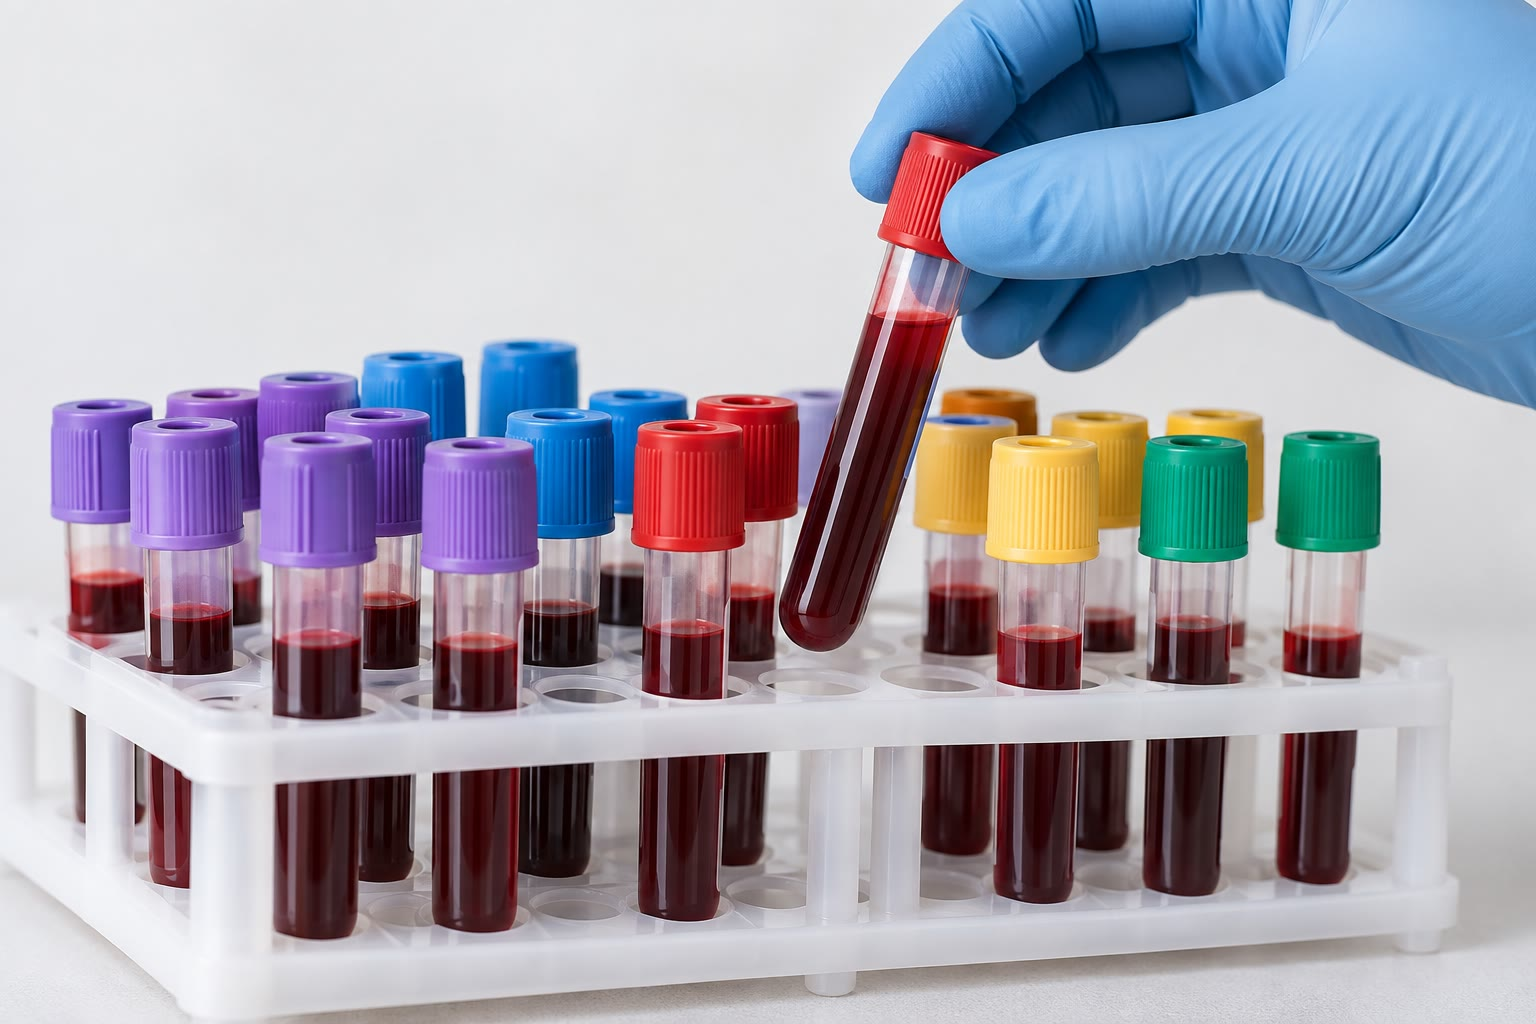
\includegraphics[width=0.45\linewidth]{images/book1/ai/g12-blood-tubes.jpg}

{\small Des échantillons de sang~: leur \omterm{def:g9:acids-bases-ph:ph}{pH} est maintenu dans un domaine
étroit.}
\end{omfigure}

\section{Les diagrammes de prédominance}

\begin{proposition}[Relation de Henderson]\label{prop:g12:buffers-predominance:henderson}
Dans toute \omterm{def:g6:solutions-and-solubility:solute}{solution aqueuse} contenant le couple \ce{HA}/\ce{A-},
\[
  \mathrm{pH} = pK_a + \log\frac{[\ce{A-}]}{[\ce{HA}]} .
\]
\end{proposition}

\begin{proof}
À partir de $K_a = \dfrac{[\ce{A-}][\ce{H3O+}]}{[\ce{HA}]c^\circ}$, on
prend $-\log$
des deux membres~: $pK_a = \mathrm{pH} - \log\dfrac{[\ce{A-}]}{[\ce{HA}]}$.
\end{proof}

\begin{definition}[Diagrammes de prédominance et de distribution]\label{def:g12:buffers-predominance:predominance}
Le \emph{diagramme de prédominance}\index{diagramme de predominance@diagramme de prédominance}
d'un couple est un axe de \omterm{def:g9:acids-bases-ph:ph}{pH} partagé en $pK_a$~: au-dessous, l'acide HA
prédomine
($[\ce{HA}] > [\ce{A-}]$)~; au-dessus, c'est la base \ce{A-}. Le
\emph{diagramme de distribution}\index{diagramme de distribution}
représente la proportion de chaque forme,
$[\ce{HA}]/c$ et $[\ce{A-}]/c$, en fonction du \omterm{def:g9:acids-bases-ph:ph}{pH}~; les deux courbes se
coupent en
$\mathrm{pH} = pK_a$.
\end{definition}

\begin{method}[Tracer un diagramme de prédominance]\label{met:g12:buffers-predominance:diagram}
\begin{enumerate}
  \item Tracer un axe de \omterm{def:g9:acids-bases-ph:ph}{pH} de 0 à 14 et y placer le $pK_a$ du couple.
  \item Écrire l'acide à gauche du $pK_a$ et la base à droite.
  \item Pour une espèce engagée dans plusieurs couples (un acide qui peut
        céder deux hydrogènes, un acide aminé), placer chaque $pK_a$~:
        chaque intervalle appartient à une forme.
  \item À une unité du $pK_a$, le rapport vaut déjà 10 pour 1~: la forme
        minoritaire représente moins de \qty{10}{\percent}.
\end{enumerate}
\end{method}

\begin{omfigure}
\begin{tikzpicture}[font=\small, x=0.62cm]
  % ledger: pka:ethanoic, pka:methanoic, kb:NH3, ka:H2CO3
  \foreach \y/\pk/\acid/\base in {0/3.74/{\ce{HCOOH}}/{\ce{HCOO-}},
      -1.0/4.76/{\ce{CH3COOH}}/{\ce{CH3COO-}}, -2.0/6.37/{\ce{CO2,H2O}}/{\ce{HCO3-}},
      -3.0/9.26/{\ce{NH4+}}/{\ce{NH3}}} {
    \fill[omThm!20] (0,\y) rectangle (\pk,\y+0.5);
    \fill[omDef!20] (\pk,\y) rectangle (14,\y+0.5);
    \draw[black!50] (0,\y) rectangle (14,\y+0.5);
    \node at (\pk/2,\y+0.25) {\acid};
    \node at ({(\pk+14)/2},\y+0.25) {\base};
    \draw[thick] (\pk,\y-0.08) -- (\pk,\y+0.58);
    \node[font=\scriptsize, anchor=south] at (\pk,\y+0.55) {\pk};
  }
  \draw[->] (0,-3.4) -- (14.5,-3.4) node[right] {pH};
  \foreach \k in {0,2,4,6,8,10,12,14} \draw (\k,-3.35) -- (\k,-3.45) node[below, font=\scriptsize] {\k};
\end{tikzpicture}

{\small \omterm{def:g12:buffers-predominance:predominance}{Diagrammes de prédominance} de quatre couples~: l'acide (à
gauche, en rouge) prédomine au-dessous de son $pK_a$, la base (à droite,
en bleu) au-dessus.}
\end{omfigure}

\begin{omfigure}
\begin{minipage}{0.49\linewidth}
\begin{tikzpicture}
\begin{axis}[width=\linewidth, height=5cm, xmin=0, xmax=14, ymin=0, ymax=1.05,
    xlabel={pH}, ylabel={proportion}, axis lines*=left, ymajorgrids,
    grid style={gray!20}, tick label style={font=\scriptsize},
    label style={font=\small}, title={\small acide éthanoïque},
    title style={yshift=-4pt}]
  \addplot[very thick, omThm] table[x=pH, y=HA] {figdata/out/grade-12-buffers-predominance-a.dat};
  \addplot[very thick, omDef] table[x=pH, y=A] {figdata/out/grade-12-buffers-predominance-a.dat};
  \addplot[dashed, black!50] coordinates {(4.76,0) (4.76,1)};
  \node[font=\scriptsize, omThm] at (axis cs:2.2,0.85) {\ce{CH3COOH}};
  \node[font=\scriptsize, omDef] at (axis cs:7.6,0.85) {\ce{CH3COO-}};
\end{axis}
\end{tikzpicture}
\end{minipage}\hfill
\begin{minipage}{0.49\linewidth}
\begin{tikzpicture}
\begin{axis}[width=\linewidth, height=5cm, xmin=0, xmax=14, ymin=0, ymax=1.05,
    xlabel={pH}, ylabel={proportion}, axis lines*=left, ymajorgrids,
    grid style={gray!20}, tick label style={font=\scriptsize},
    label style={font=\small}, title={\small glycine},
    title style={yshift=-4pt}]
  \addplot[very thick, omThm] table[x=pH, y=cation] {figdata/out/grade-12-buffers-predominance-b.dat};
  \addplot[very thick, omMeth] table[x=pH, y=zwitterion] {figdata/out/grade-12-buffers-predominance-b.dat};
  \addplot[very thick, omDef] table[x=pH, y=anion] {figdata/out/grade-12-buffers-predominance-b.dat};
  \node[font=\scriptsize, omThm] at (axis cs:1.0,0.55) {cation};
  \node[font=\scriptsize, omMeth] at (axis cs:6.1,0.88) {zwitterion};
  \node[font=\scriptsize, omDef] at (axis cs:12.6,0.55) {anion};
\end{axis}
\end{tikzpicture}
\end{minipage}

{\small \omterm{def:g12:buffers-predominance:predominance}{Diagrammes de distribution}, calculés à partir des valeurs de
$pK_a$. À gauche~: l'acide éthanoïque, les courbes se coupent à 4.76. À
droite~: la glycine,
\ce{H2N-CH2-COOH}, avec deux couples ($pK_a$ 2.35 et 9.78)~: le \omterm{def:g9:ions:ion}{cation}
\ce{H3N+-CH2-COOH}, le zwitterion \ce{H3N+-CH2-COO-} et l'\omterm{def:g9:ions:ion}{anion}
\ce{H2N-CH2-COO-}.}
\end{omfigure}

\begin{example}[La glycine dans l'organisme]\label{ex:g12:buffers-predominance:glycine}
% ledger: pka:glycine1, pka:glycine2, ph:blood
Au \omterm{def:g9:acids-bases-ph:ph}{pH} du sang, environ 7.4, la glycine se situe entre ses deux valeurs
de $pK_a$~: elle est presque entièrement sous forme de zwitterion,
portant une charge positive sur son azote et une charge négative sur son
groupe carboxylate, et globalement neutre. Tous les acides aminés se
comportent de la même façon.
\end{example}

\section{Les indicateurs colorés}


\begin{definition}[Indicateur coloré acido-basique, zone de virage]\label{def:g12:buffers-predominance:indicator}
Un \emph{indicateur coloré acido-basique}\index{indicateur colore acido-basique@indicateur coloré acido-basique}
est un couple \ce{HInd}/\ce{Ind-} dont les deux formes ont des couleurs
différentes, utilisé en très petite quantité. Sa \emph{zone de
virage}\index{zone de virage} est l'intervalle de \omterm{def:g9:acids-bases-ph:ph}{pH} sur lequel on voit
la couleur changer, à peu près de
$pK_a - 1$ à $pK_a + 1$~: au-dessous, on voit la couleur de \ce{HInd},
au-dessus, celle de \ce{Ind-}, et entre les deux un \omterm{def:g6:pure-substances-and-mixtures:mixture}{mélange} des deux.
\end{definition}

\begin{omfigure}
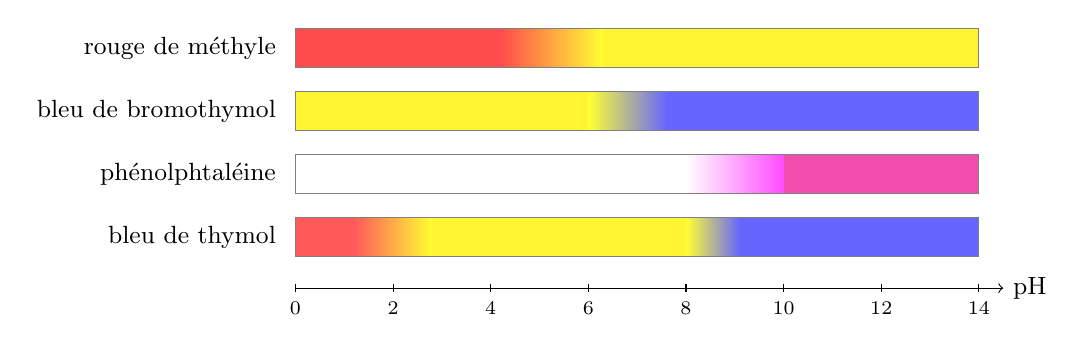
\begin{tikzpicture}[font=\small, x=0.62cm]
  % ledger: ind:methyl-red, ind:BBT, ind:phenolphthalein, ind:thymol-blue, ind:range-rule
  \foreach \y/\name/\a/\b/\ca/\cm/\cb in {
      0/{rouge de méthyle}/4.2/6.3/red!70/orange/yellow!80,
      -0.8/{bleu de bromothymol}/6.0/7.6/yellow!80/green!60/blue!60,
      -1.6/{phénolphtaléine}/8.0/10.0/white/magenta!25/magenta!70} {
    \fill[\ca] (0,\y) rectangle (\a,\y+0.5);
    \shade[left color=\ca, right color=\cb] (\a,\y) rectangle (\b,\y+0.5);
    \fill[\cb] (\b,\y) rectangle (14,\y+0.5);
    \draw[black!50] (0,\y) rectangle (14,\y+0.5);
    \node[anchor=east] at (-0.2,\y+0.25) {\name};
  }
  \fill[red!65] (0,-2.4) rectangle (1.2,-1.9);
  \shade[left color=red!65, right color=yellow!80] (1.2,-2.4) rectangle (2.8,-1.9);
  \fill[yellow!80] (2.8,-2.4) rectangle (8.0,-1.9);
  \shade[left color=yellow!80, right color=blue!60] (8.0,-2.4) rectangle (9.1,-1.9);
  \fill[blue!60] (9.1,-2.4) rectangle (14,-1.9);
  \draw[black!50] (0,-2.4) rectangle (14,-1.9);
  \node[anchor=east] at (-0.2,-2.15) {bleu de thymol};
  \draw[->] (0,-2.8) -- (14.5,-2.8) node[right] {pH};
  \foreach \k in {0,2,4,6,8,10,12,14} \draw (\k,-2.75) -- (\k,-2.85) node[below, font=\scriptsize] {\k};
\end{tikzpicture}

{\small Couleurs de quatre indicateurs en fonction du \omterm{def:g9:acids-bases-ph:ph}{pH}~; les parties
dégradées sont les \omterm{def:g12:buffers-predominance:indicator}{zones de virage}. Le bleu de thymol, qui possède deux
couples, a deux \omterm{def:g12:buffers-predominance:indicator}{zones de virage}.}
\end{omfigure}

\begin{method}[Choisir un indicateur]\label{met:g12:buffers-predominance:indicator}
Pour repérer le moment où une solution franchit un \omterm{def:g9:acids-bases-ph:ph}{pH} donné (le \omterm{def:g9:acids-bases-ph:ph}{pH} à la
fin d'un \omterm{def:g11:titration:titration}{titrage}, par exemple), choisir un indicateur dont la \omterm{def:g12:buffers-predominance:indicator}{zone de
virage} contient ce \omterm{def:g9:acids-bases-ph:ph}{pH}~: la couleur change alors exactement à cet
endroit.
\end{method}

\section{Les solutions tampons}

\begin{definition}[Solution tampon]\label{def:g12:buffers-predominance:buffer}
Une \emph{solution tampon}\index{solution tampon} est une solution dont
le \omterm{def:g9:acids-bases-ph:ph}{pH} varie très peu quand on y ajoute un peu d'acide ou de base, ou
quand on la dilue. Elle est en général constituée d'un \omterm{def:g12:ka-and-pka:strong-acid}{acide faible} et
de sa base conjuguée en quantités comparables~; son \omterm{def:g9:acids-bases-ph:ph}{pH} est alors voisin
du $pK_a$ du couple.
\end{definition}

\begin{proposition}[Pourquoi un tampon résiste]\label{prop:g12:buffers-predominance:buffer}
Dans un tampon de \ce{HA} et \ce{A-}, un \omterm{def:g12:ka-and-pka:strong-acid}{acide fort} ajouté est consommé
par
\ce{A-} (\ce{A- + H3O+ -> HA + H2O}) et une \omterm{def:g12:ka-and-pka:strong-acid}{base forte} ajoutée par
\ce{HA}
(\ce{HA + OH- -> A- + H2O})~; le rapport $[\ce{A-}]/[\ce{HA}]$, et donc
le \omterm{def:g9:acids-bases-ph:ph}{pH}, ne varie que peu. La \omterm{def:g10:concentration-and-dilution:dilution}{dilution} ne change pas du tout le rapport.
\end{proposition}

\begin{proof}
D'après la relation de Henderson, le \omterm{def:g9:acids-bases-ph:ph}{pH} ne dépend que du rapport.
Ajouter \qty{1}{mmol} d'acide à un tampon qui contient \qty{10}{mmol} de
chaque forme fait passer le rapport de $10/10$ à $9/11$, et ne modifie
le \omterm{def:g9:acids-bases-ph:ph}{pH} que de
$\log(9/11) = -0.09$.
\end{proof}

\begin{omfigure}
\begin{tikzpicture}
\begin{axis}[width=0.75\linewidth, height=5.6cm, xmin=0, xmax=10, ymin=0,
    ymax=8, xlabel={volume de \ce{HCl} à \qty{0.10}{mol/L} ajouté (\si{mL})},
    ylabel={pH}, axis lines*=left, ymajorgrids, grid style={gray!20},
    tick label style={font=\small}, label style={font=\small},
    legend style={font=\small, at={(0.98,0.97)}, anchor=north east,
    draw=none, fill=white}, legend cell align=left]
  % ledger: pka:ethanoic (buffer recipe: exercise data)
  \addplot[very thick, omThm, mark=*, mark size=1.3pt] table[x=V, y=water]
    {figdata/out/grade-12-buffers-predominance-c.dat};
  \addplot[very thick, omDef, mark=*, mark size=1.3pt] table[x=V, y=buffer]
    {figdata/out/grade-12-buffers-predominance-c.dat};
  \legend{\qty{100}{mL} d'eau pure, \qty{100}{mL} de tampon éthanoate}
\end{axis}
\end{tikzpicture}

{\small Ajout d'acide chlorhydrique à de l'eau pure et à un tampon
d'acide éthanoïque et d'éthanoate de sodium (\qty{0.10}{mol/L} de
chaque). Le \omterm{def:g9:acids-bases-ph:ph}{pH} de l'eau passe de 7 à environ 2~; celui du tampon, de
4.76 à 4.67.}
\end{omfigure}

\begin{method}[Préparer un tampon]\label{met:g12:buffers-predominance:prepare}
\begin{enumerate}
  \item Choisir un couple dont le $pK_a$ est à moins d'une unité du \omterm{def:g9:acids-bases-ph:ph}{pH}
        voulu (idéalement très proche).
  \item Calculer le rapport $[\ce{A-}]/[\ce{HA}] = 10^{\mathrm{pH} - pK_a}$.
  \item \omterm{def:g2:mixing-and-dissolving:mix}{Mélanger} l'\omterm{def:g12:ka-and-pka:strong-acid}{acide faible} et un sel de sa base dans ce rapport, à
        des concentrations assez élevées pour absorber les quantités
        d'acide ou de base apportées.
\end{enumerate}
\end{method}

\begin{inthelab}[Préparer un tampon à pH 4.8]
On \omterm{def:g6:pure-substances-and-mixtures:mixture}{mélange} \qty{50.0}{mL} d'acide éthanoïque à \qty{0.10}{mol/L} avec
\qty{50.0}{mL} d'éthanoate de sodium à \qty{0.10}{mol/L}~; le \omterm{def:g9:acids-bases-ph:ph-paper}{pH-mètre}
indique environ 4.8. Quelques gouttes d'acide chlorhydrique à
\qty{1}{mol/L} modifient à peine la mesure, alors que les mêmes gouttes
dans \qty{100}{mL} d'eau distillée la font descendre vers 3.
\end{inthelab}

\section{Les tampons du vivant}

\begin{example}[Le tampon du sang]\label{ex:g12:buffers-predominance:blood}
% ledger: pk:blood-bicarb, ph:blood, hco3:blood
Le principal tampon du sang est le couple formé du dioxyde de carbone
dissous et de l'\omterm{def:g9:ions:ion}{ion} hydrogénocarbonate, \ce{CO2,H2O}/\ce{HCO3-}. Dans le
sang, les physiologistes utilisent pour ce couple la relation
$\mathrm{pH} = 6.1 +
\log\big([\ce{HCO3-}]/[\ce{CO2}]\big)$. Les poumons éliminent le dioxyde
de carbone, les reins ajustent l'hydrogénocarbonate~: ensemble, ils
maintiennent le rapport, et donc le \omterm{def:g9:acids-bases-ph:ph}{pH}.
\end{example}

\begin{omfigure}
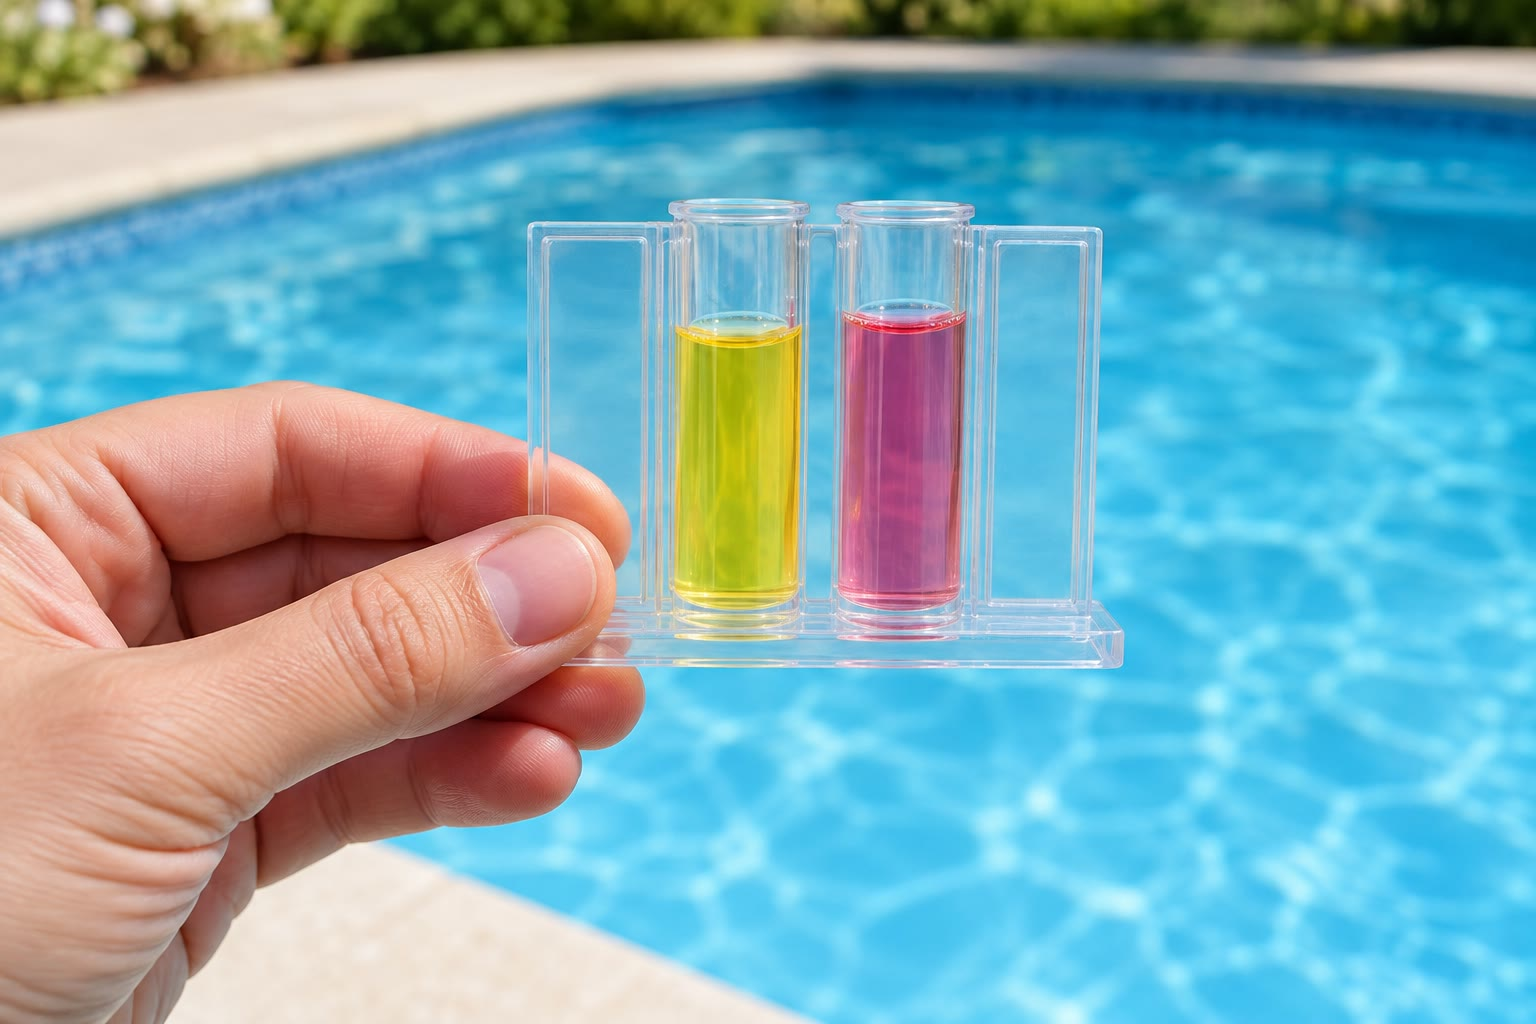
\includegraphics[width=0.45\linewidth]{images/book1/ai/g12-pool-test.jpg}

{\small Analyse de l'eau d'une piscine~: les couleurs des indicateurs
donnent le \omterm{def:g9:acids-bases-ph:ph}{pH}.}
\end{omfigure}

\section{Exercices}


\begin{exercise}[$\star$]\label{exo:g12:buffers-predominance:1}
Quelle forme du couple \ce{CH3COOH}/\ce{CH3COO-} ($pK_a = 4.76$)
prédomine à \omterm{def:g9:acids-bases-ph:ph}{pH} 2, à \omterm{def:g9:acids-bases-ph:ph}{pH} 4.76 et à \omterm{def:g9:acids-bases-ph:ph}{pH} 7~?
\end{exercise}

\begin{exercise}[$\star$]\label{exo:g12:buffers-predominance:2}
Sur le \omterm{def:g12:buffers-predominance:predominance}{diagramme de distribution} de l'acide éthanoïque, lire la
proportion de
\ce{CH3COO-} à \omterm{def:g9:acids-bases-ph:ph}{pH} 4 et à \omterm{def:g9:acids-bases-ph:ph}{pH} 6.
\end{exercise}

\begin{exercise}[$\star$]\label{exo:g12:buffers-predominance:3}
Quelle couleur prend le bleu de bromothymol à \omterm{def:g9:acids-bases-ph:ph}{pH} 5~? À \omterm{def:g9:acids-bases-ph:ph}{pH} 7~? À \omterm{def:g9:acids-bases-ph:ph}{pH} 9~?
\end{exercise}

\begin{exercise}[$\star$]\label{exo:g12:buffers-predominance:4}
Quelle forme du couple \ce{NH4+}/\ce{NH3} prédomine dans une solution à
\omterm{def:g9:acids-bases-ph:ph}{pH} 7.4~? À \omterm{def:g9:acids-bases-ph:ph}{pH} 11~?
\end{exercise}

\begin{exercise}[$\star$]\label{exo:g12:buffers-predominance:5}
Pourquoi utilise-t-on les indicateurs en très petite quantité~?
\end{exercise}

\begin{exercise}[$\star\star$]\label{exo:g12:buffers-predominance:6}
Calculer le rapport $[\ce{CH3COO-}]/[\ce{CH3COOH}]$ à \omterm{def:g9:acids-bases-ph:ph}{pH} 3.76, 4.76 et
5.76.
\end{exercise}

\begin{exercise}[$\star\star$]\label{exo:g12:buffers-predominance:7}
Un \omterm{def:g11:titration:titration}{titrage} se termine à \omterm{def:g9:acids-bases-ph:ph}{pH} 8.7. Lequel des quatre indicateurs de la
figure choisir~? Pourquoi pas le rouge de méthyle~?
\end{exercise}

\begin{exercise}[$\star\star$]\label{exo:g12:buffers-predominance:8}
Un tampon contient \qty{0.20}{mol/L} d'acide éthanoïque et
\qty{0.10}{mol/L} d'éthanoate de sodium. Calculer son \omterm{def:g9:acids-bases-ph:ph}{pH}.
\end{exercise}

\begin{exercise}[$\star\star$]\label{exo:g12:buffers-predominance:9}
À l'aide du diagramme de la glycine, donner la forme prédominante à \omterm{def:g9:acids-bases-ph:ph}{pH}
1, 6 et 12, avec sa charge.
\end{exercise}

\begin{exercise}[$\star\star$]\label{exo:g12:buffers-predominance:10}
Lire les courbes de réponse~: de combien le \omterm{def:g9:acids-bases-ph:ph}{pH} de l'eau diminue-t-il
après ajout de
\qty{1.0}{mL} d'acide~? Et celui du tampon~?
\end{exercise}

\begin{exercise}[$\star\star$]\label{exo:g12:buffers-predominance:11}
Quel couple de la figure des \omterm{def:g12:buffers-predominance:predominance}{diagrammes de prédominance} choisir pour
préparer un tampon à \omterm{def:g9:acids-bases-ph:ph}{pH} 9.5~? Dans quel rapport \omterm{def:g2:mixing-and-dissolving:mix}{mélanger} ses deux
formes~?
\end{exercise}

\begin{exercise}[$\star\star\star$]\label{exo:g12:buffers-predominance:12}
Le tampon éthanoate de la figure (\qty{10}{mmol} de chaque forme) reçoit
de l'acide chlorhydrique. Quelle quantité d'acide peut-il recevoir avant
que son \omterm{def:g9:acids-bases-ph:ph}{pH} ait diminué d'une unité~? Pourquoi dit-on qu'un tampon plus
concentré a un plus grand pouvoir tampon~?
\end{exercise}

\begin{exercise}[$\star\star\star$]\label{exo:g12:buffers-predominance:13}
Quel volume de solution d'éthanoate de sodium à \qty{0.10}{mol/L} faut-il
ajouter à \qty{100}{mL} d'acide éthanoïque à \qty{0.10}{mol/L} pour
obtenir un tampon à \omterm{def:g9:acids-bases-ph:ph}{pH} 5.0~?
\end{exercise}

\begin{exercise}[$\star\star\star$]\label{exo:g12:buffers-predominance:14}
Le bleu de thymol a deux \omterm{def:g12:buffers-predominance:indicator}{zones de virage}. Expliquer pourquoi, et donner
sa couleur à \omterm{def:g9:acids-bases-ph:ph}{pH} 1, 5 et 10.
\end{exercise}

\begin{exercise}[$\star\star\star$]\label{exo:g12:buffers-predominance:15}
Un tampon à \omterm{def:g9:acids-bases-ph:ph}{pH} 4.76 est dilué dix fois avec de l'eau distillée. Quel est
son nouveau \omterm{def:g9:acids-bases-ph:ph}{pH}, d'après la relation de Henderson~? Que se passe-t-il si
l'on dilue dix fois un \omterm{def:g12:ka-and-pka:strong-acid}{acide fort} de même \omterm{def:g9:acids-bases-ph:ph}{pH}~?
\end{exercise}

\section{Problème~: le tampon du sang}

\begin{problem}[{Problème du week-end --- quel rapport entre
hydrogénocarbonate et dioxyde de carbone maintient le sang à pH 7.4~?}]
\label{pb:g12:buffers-predominance:1}
% ledger: pk:blood-bicarb, ph:blood, hco3:blood
Le \omterm{def:g9:acids-bases-ph:ph}{pH} du sang artériel est normalement compris entre 7.38 et 7.42. Son
principal tampon est le couple \ce{CO2,H2O}/\ce{HCO3-}, pour lequel les
physiologistes utilisent
$\mathrm{pH} = 6.1 + \log\big([\ce{HCO3-}]/[\ce{CO2}]\big)$. La
concentration normale du sang en hydrogénocarbonate est de 22 à
\qty{28}{mmol/L}.

\medskip
\noindent\textbf{Partie I --- Le couple.}
\begin{enumerate}
  \item Écrire la réaction du dioxyde de carbone dissous avec l'eau qui
        donne des \omterm{def:g9:ions:ion}{ions} hydrogénocarbonate.
  \item Quelle espèce est l'acide, laquelle est la base~?
  \item La valeur 6.1 diffère du 6.37 de la table des $pK_a$. En donner
        une raison (penser à la température du corps et aux autres \omterm{def:g9:ions:ion}{ions}
        présents).
  \item Quelle quantité d'hydrogénocarbonate \qty{5.0}{L} de sang
        contiennent-ils à \qty{24}{mmol/L}~?
\end{enumerate}

\medskip
\noindent\textbf{Partie II --- Prédominance.}
\begin{enumerate}[resume]
  \item Tracer le \omterm{def:g12:buffers-predominance:predominance}{diagramme de prédominance} du couple avec $pK = 6.1$.
  \item Quelle forme prédomine dans le sang~?
  \item Le sang est-il légèrement acide ou légèrement basique~?
\end{enumerate}

\medskip
\noindent\textbf{Partie III --- Le rapport.}
\begin{enumerate}[resume]
  \item À l'aide de la relation, calculer le rapport
        $[\ce{HCO3-}]/[\ce{CO2}]$
        à \omterm{def:g9:acids-bases-ph:ph}{pH} 7.4.
  \item Avec $[\ce{HCO3-}] = \qty{24}{mmol/L}$, calculer $[\ce{CO2}]$.
  \item Calculer le rapport aux deux extrémités du domaine normal, 7.38
        et 7.42.
  \item Quelle fraction du couple est sous forme d'hydrogénocarbonate à
        \omterm{def:g9:acids-bases-ph:ph}{pH} 7.4~?
  \item Un sang trop basique peut atteindre un \omterm{def:g9:acids-bases-ph:ph}{pH} de 7.6. Que vaut alors
        le rapport~?
\end{enumerate}

\medskip
\noindent\textbf{Partie IV --- Quand l'équilibre est rompu.}
\begin{enumerate}[resume]
  \item Lors d'un effort intense, des acides entrent dans le sang. Quelle
        forme du couple les consomme~? Écrire la réaction.
  \item Si le \omterm{def:g9:acids-bases-ph:ph}{pH} descendait à 7.1, que deviendrait le rapport~?
  \item À hydrogénocarbonate inchangé, de combien le dioxyde de carbone
        devrait-il augmenter~? Que font les poumons pour réagir~?
  \item Pourquoi un \omterm{def:g12:ka-and-pka:strong-acid}{acide faible} associé à sa base, plutôt qu'un \omterm{def:g12:ka-and-pka:strong-acid}{acide
        fort}, est-il le bon outil pour maintenir un \omterm{def:g9:acids-bases-ph:ph}{pH}~?
  \item De combien le \omterm{def:g9:acids-bases-ph:ph}{pH} varie-t-il si les deux concentrations sont
        divisées par deux~? Pourquoi~?
  \item Donner la réponse finale~: quel est le rapport entre
        hydrogénocarbonate et dioxyde de carbone dans le sang à \omterm{def:g9:acids-bases-ph:ph}{pH} 7.4~?
\end{enumerate}
\end{problem}
